\documentclass[aspectratio=169,10pt]{beamer}
\usepackage[T1]{fontenc}
\usepackage{lmodern}
\usepackage{amsmath,booktabs,graphicx,tikz}
\usetikzlibrary{arrows.meta,positioning,calc,fit,backgrounds}
\definecolor{Ink}{HTML}{11181D}
\definecolor{Panel}{HTML}{1C292F}
\definecolor{Lime}{HTML}{CBF268}
\definecolor{Mist}{HTML}{EAF1F2}
\definecolor{Muted}{HTML}{A7BDC5}
\definecolor{Cyan}{HTML}{69CBCD}
\setbeamercolor{background canvas}{bg=Ink}
\setbeamercolor{normal text}{fg=Mist,bg=Ink}
\setbeamercolor{frametitle}{fg=Lime}
\setbeamercolor{title}{fg=Lime}
\setbeamercolor{structure}{fg=Lime}
\setbeamercolor{block title}{fg=Ink,bg=Lime}
\setbeamercolor{block body}{fg=Mist,bg=Panel}
\setbeamercolor{itemize item}{fg=Lime}
\setbeamercolor{itemize subitem}{fg=Cyan}
\setbeamercolor{footline}{fg=Muted}
\setbeamertemplate{navigation symbols}{}
\setbeamertemplate{itemize items}[circle]
\setbeamertemplate{footline}{\hspace{5mm}\scriptsize CURIOSITY AFTERSHOCKS\hfill BIG DATA ANALYTICS\hspace{6mm}\insertframenumber/\inserttotalframenumber\hspace{5mm}\vspace{3mm}}
\setbeamersize{text margin left=9mm,text margin right=9mm}
\setbeamerfont{frametitle}{size=\Large,series=\bfseries}
\setbeamerfont{title}{size=\huge,series=\bfseries}
\hypersetup{colorlinks=true,urlcolor=Cyan,linkcolor=Lime}
\pdfstringdefDisableCommands{\def\quad{ }\def\texttt#1{#1}}
\graphicspath{{assets/}{../}}
\newcommand{\takeaway}[1]{\vfill{\color{Lime}\small #1}}
\newcommand{\source}[1]{{\color{Muted}\tiny #1}}
\tikzset{box/.style={draw=Muted,fill=Panel,rounded corners=3pt,align=center,text=Mist,minimum height=9mm,font=\small},arr/.style={-{Latex[length=2mm]},thick,draw=Lime},msg/.style={-{Latex[length=1.5mm]},draw=Lime},life/.style={dashed,draw=Muted!60}}
\title{Curiosity Aftershocks}
\subtitle{Discovering unexpected attention spikes\texorpdfstring{\\}{ }after real-world events}
\author{}
\institute{}
\begin{document}

\begin{frame}[plain]
\vspace{8mm}
{\color{Muted}\small A BIG DATA ANALYTICS PROJECT}\par\vspace{8mm}
{\usebeamerfont{title}\color{Lime}\inserttitle}\par\vspace{4mm}
{\Large\insertsubtitle}\par\vspace{9mm}
{\color{Cyan}The world happens. Curiosity ripples.}\par\vfill

{\scriptsize\color{Muted}\insertdate}
\end{frame}

\begin{frame}{Problem statement}
\begin{block}{The exact problem we address}
Given a recent event and its time, automatically identify English Wikipedia topics whose hourly views rise unusually above their pre-event levels, without selecting topics in advance. Show these topics and their shared traffic patterns in an interactive graph using freely available data.
\end{block}
\vspace{4mm}
\textbf{Why this problem matters}
\begin{itemize}\setlength\itemsep{3mm}
\item A fixed topic list can miss unexpected changes in public interest.
\item High view counts alone do not tell us whether attention is unusual.
\item Millions of records per hour require automated processing.
\end{itemize}
\takeaway{We detect changes after an event; we do not claim that the event caused them.}
\end{frame}

\begin{frame}{Our solution and the tools we use}
\textbf{Enter an event time $\rightarrow$ detect traffic spikes $\rightarrow$ explore the graph.}
\vspace{4mm}
\renewcommand{\arraystretch}{1.25}
\begin{tabular}{p{5.2cm}p{7.3cm}}
\toprule
\textbf{Tool / technology} & \textbf{Role in our solution}\\\midrule
Python + Apache Spark & Read millions of records and calculate traffic spikes.\\
Spark Structured Streaming & Process newly available hourly data files.\\
Apache Parquet & Store processed hourly data for efficient reuse.\\
NumPy & Compare topic traffic patterns to create graph links.\\
FastAPI & Provide start/stop controls and analytical results.\\
React + TypeScript & Display the interactive dashboard and topic graph.\\\bottomrule
\end{tabular}
\takeaway{A separate historical view uses Spark MLlib to group similar response patterns.}
\end{frame}

\begin{frame}{Data source: free Wikipedia pageview counts}
\begin{itemize}\setlength\itemsep{4mm}
\item \textbf{Source:} public hourly files from Wikimedia; no account or API key.
\item \textbf{Information used:} article title, hour, and number of views.
\item \textbf{Scope:} English Wikipedia desktop and mobile traffic; system pages excluded.
\item \textbf{Traceability:} source links, file checksums, and timestamps are saved.
\item \textbf{Cost:} no paid dataset; processing uses local storage and computing resources.
\end{itemize}
\takeaway{Files arrive with a delay and may include automated traffic.}
\par\vspace{2mm}\source{Dataset: \url{https://dumps.wikimedia.org/other/pageviews/}. Source records: docs/live-source-manifest.json.}
\end{frame}

\begin{frame}{System architecture: how the components connect}
\centering
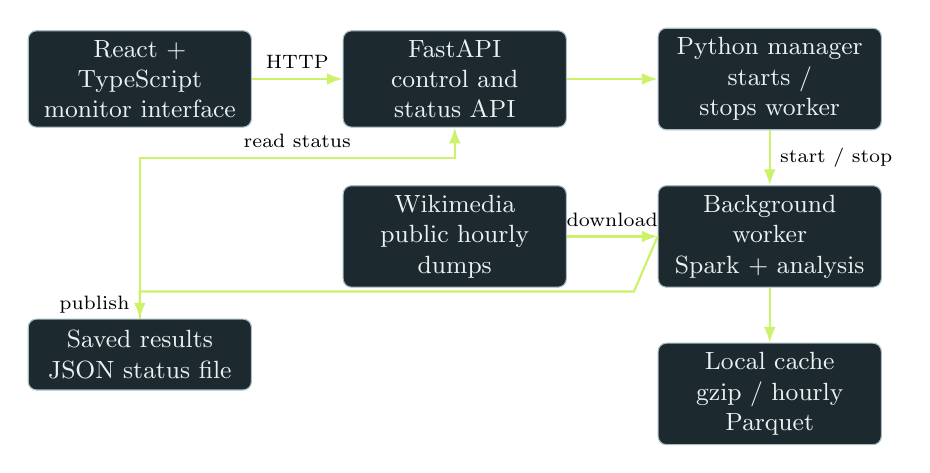
\begin{tikzpicture}[node distance=9mm]
\node[box,text width=2.6cm] (ui) at (0,0) {React + TypeScript\\monitor interface};
\node[box,text width=2.6cm] (api) at (4,0) {FastAPI\\control and status API};
\node[box,text width=2.6cm] (mgr) at (8,0) {Python manager\\starts / stops worker};
\node[box,text width=2.6cm] (worker) at (8,-2) {Background worker\\Spark + analysis};
\node[box,text width=2.6cm] (source) at (4,-2) {Wikimedia\\public hourly dumps};
\node[box,text width=2.6cm] (cache) at (8,-4) {Local cache\\gzip / hourly Parquet};
\node[box,text width=2.6cm] (state) at (0,-3.5) {Saved results\\JSON status file};
\draw[arr] (ui)--node[above,font=\scriptsize]{HTTP}(api);
\draw[arr] (api)--(mgr);
\draw[arr] (mgr)--node[right,font=\scriptsize]{start / stop}(worker);
\draw[arr] (source)--node[above,font=\scriptsize]{download}(worker);
\draw[arr] (worker)--(cache);
\draw[arr] (worker.west)--++(-.3,-.7)-|node[pos=.75,left,font=\scriptsize]{publish}(state.north);
\draw[arr] (state.north)--(0,-1)--node[above,font=\scriptsize]{read status}(4,-1)--(api.south);
\end{tikzpicture}
\takeaway{Spark processes data in the background while the interface stays responsive.}
\end{frame}

\begin{frame}{Data flow: from hourly files to the graph}
\centering
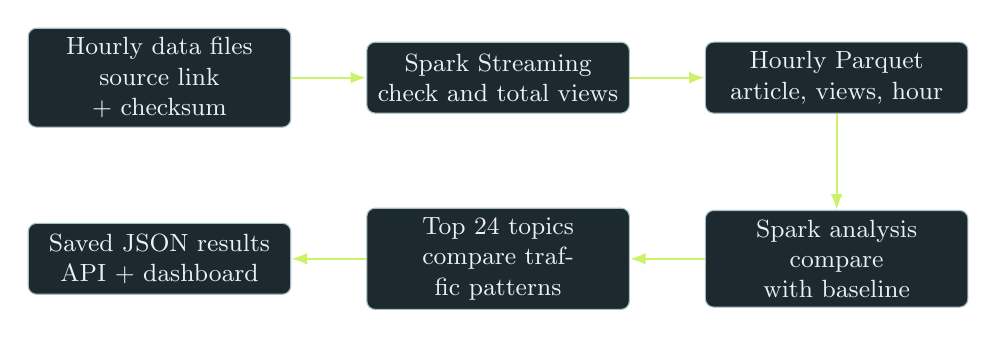
\begin{tikzpicture}
\node[box,text width=3.1cm] (a) at (0,0) {Hourly data files\\source link + checksum};
\node[box,text width=3.1cm] (b) at (4.3,0) {Spark Streaming\\check and total views};
\node[box,text width=3.1cm] (c) at (8.6,0) {Hourly Parquet\\article, views, hour};
\node[box,text width=3.1cm] (d) at (8.6,-2.3) {Spark analysis\\compare with baseline};
\node[box,text width=3.1cm] (e) at (4.3,-2.3) {Top 24 topics\\compare traffic patterns};
\node[box,text width=3.1cm] (f) at (0,-2.3) {Saved JSON results\\API + dashboard};
\foreach \u/\v in {a/b,b/c,c/d,d/e,e/f}{\draw[arr] (\u)--(\v);}
\end{tikzpicture}
\vspace{5mm}
\begin{itemize}
\item Spark reads the full files and scores eligible articles.
\item Only the top 24 candidates are compared to build the graph.
\item Saved Parquet data avoids processing the same source files again.
\end{itemize}
\end{frame}

\begin{frame}{System sequence: event to discovery}
\centering
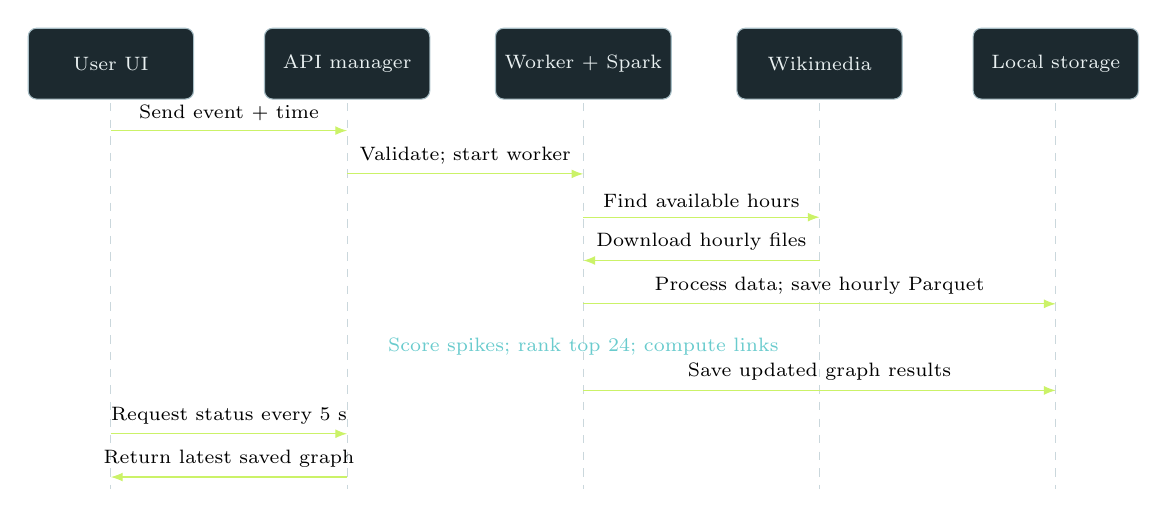
\begin{tikzpicture}[x=1cm,y=1cm,font=\scriptsize]
\foreach \x/\name in {0/User UI,3/API manager,6/Worker + Spark,9/Wikimedia,12/Local storage}{
\node[box,font=\scriptsize,minimum width=2.1cm] at (\x,0) {\name};
\draw[life] (\x,-.5)--(\x,-5.4);}
\draw[msg] (0,-.85)--node[above]{Send event + time}(3,-.85);
\draw[msg] (3,-1.4)--node[above]{Validate; start worker}(6,-1.4);
\draw[msg] (6,-1.95)--node[above]{Find available hours}(9,-1.95);
\draw[msg] (9,-2.5)--node[above]{Download hourly files}(6,-2.5);
\draw[msg] (6,-3.05)--node[above]{Process data; save hourly Parquet}(12,-3.05);
\node[text=Cyan,align=center] at (6,-3.6) {Score spikes; rank top 24; compute links};
\draw[msg] (6,-4.15)--node[above]{Save updated graph results}(12,-4.15);
\draw[msg] (0,-4.7)--node[above]{Request status every 5 s}(3,-4.7);
\draw[msg] (3,-5.25)--node[above]{Return latest saved graph}(0,-5.25);
\end{tikzpicture}
\takeaway{Worker checks new files every 5 minutes. Missing data produces a visible waiting state.}
\end{frame}

\begin{frame}{How we detect a sudden rise in attention}
\textbf{Baseline:} an article's average views in the three hours before the event hour.
\vspace{3mm}
\begin{columns}[T]
\column{.48\textwidth}
\begin{block}{Two easy-to-read measures}
\[
\text{Lift}=\frac{\text{current views}}{\text{baseline average}}
\]
\[
\text{Excess}=\text{current views}-\text{baseline average}
\]
\end{block}
\small\textbf{Illustration:} baseline 100, current 400\\
$\Rightarrow$ lift $=4\times$; excess $=300$ views.
\column{.48\textwidth}
\textbf{A candidate must pass every rule}
\begin{itemize}\setlength\itemsep{2mm}
\item All three baseline hours available.
\item Baseline average $\geq10$ views/hour.
\item Current views $\geq200$.
\item Lift $\geq3\times$ and excess $\geq100$.
\item Burst score $\geq4$.
\end{itemize}
\end{columns}
\vspace{2mm}
\small Burst score $=\dfrac{\text{Excess}}{\max(\sigma,\sqrt{\mu},1)}$, where $\mu$ is the baseline average and $\sigma$ its standard deviation.
\takeaway{The burst score measures growth relative to baseline variation; it is not a probability.}
\end{frame}

\begin{frame}{Graph construction: what does a link mean?}
\begin{columns}[T]
\column{.64\textwidth}
\begin{itemize}\setlength\itemsep{3mm}
\item Each node is a topic; show up to 24 with the largest excess views.
\item Compare two topics only at hours observed for both.
\item Use $\log(1+\text{views})$ to reduce the influence of very large counts.
\item Draw a link when their patterns are strongly similar: correlation $r\geq0.85$ across at least five shared hours.
\item Missing observations are not replaced with zeros.
\end{itemize}
\column{.32\textwidth}
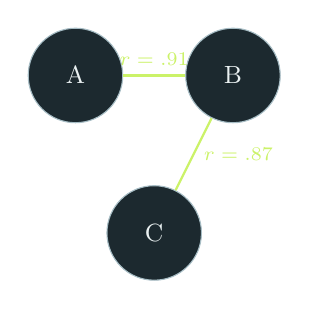
\begin{tikzpicture}
\node[box,circle,minimum size=12mm] (a) at (0,0) {A};
\node[box,circle,minimum size=12mm] (b) at (2,0) {B};
\node[box,circle,minimum size=12mm] (c) at (1,-2) {C};
\draw[thick,Lime] (a)--node[above,font=\scriptsize]{$r=.91$}(b);
\draw[thick,Lime] (b)--node[right,font=\scriptsize]{$r=.87$}(c);
\end{tikzpicture}
\source{Illustrative graph}
\end{columns}
\takeaway{A link means the traffic patterns move together; it does not prove a causal connection.}
\end{frame}

\begin{frame}{Interface: from discovery to inspection}
\centering
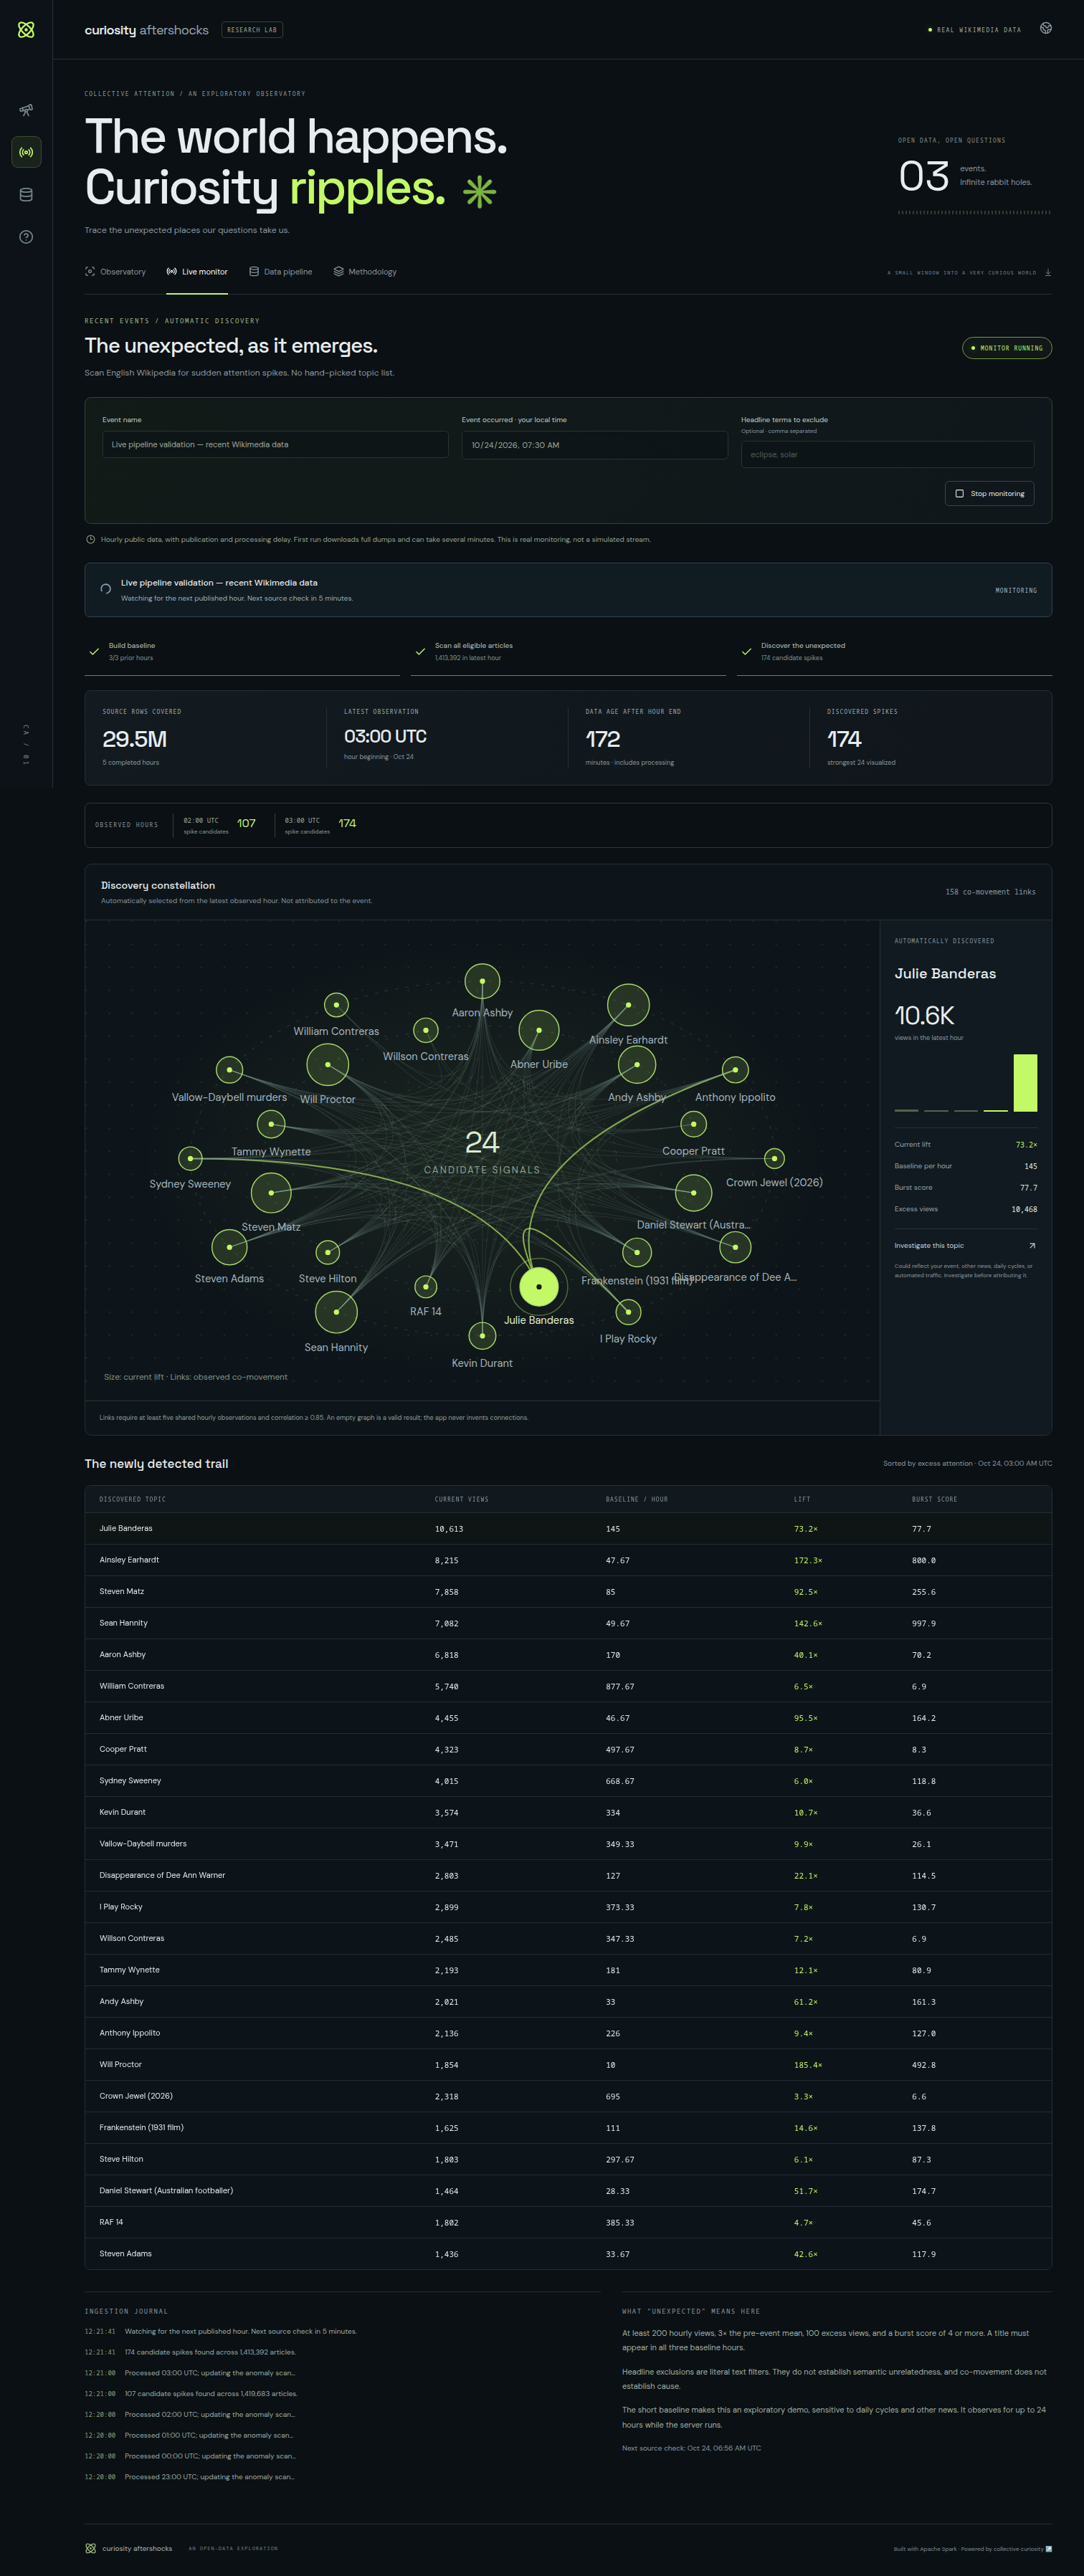
\includegraphics[width=.89\textwidth,height=5.65cm,keepaspectratio]{live-monitor.png}
\par\source{Actual validation watch: docs/live-monitor.png. Saved screenshot, not a current live feed.}
\end{frame}

\begin{frame}{Measured validation: 29.5 million records}
\begin{columns}[T]
\column{.45\textwidth}
{\Huge\color{Lime}29,509,818}\par\medskip
Source records across five complete hourly files\par\bigskip
\textbf{Validation window}\par
23 Oct 2026, 23:00 UTC through\\24 Oct 2026, 03:00 UTC\par\medskip
Three baseline hours + two observed hours
\column{.51\textwidth}
\begin{tabular}{lrr}
\toprule
\textbf{Observed hour} & \textbf{02:00} & \textbf{03:00}\\\midrule
English titles & 1,419,683 & 1,413,392\\[2mm]
Spike candidates & 107 & 174\\\bottomrule
\end{tabular}
\bigskip\par
Latest graph: \textbf{24 nodes, 158 links}\par\medskip
Initial fresh-data warm-up: approximately \textbf{20 minutes} on the validation connection.
\end{columns}
\vspace{3mm}\par
\small\textbf{Verification:} 17 backend/analytics tests and 5 browser tests passed; production build passed.
\takeaway{This validates the pipeline; it does not link these spikes to a specific news event.}\par
\source{Evidence: docs/live-validation.json; docs/live-source-manifest.json; docs/VERIFICATION.md.}
\end{frame}
\end{document}
